\hypertarget{sh__init_8c}{
\section{sh\_\-init.c File Reference}
\label{sh__init_8c}\index{sh_init.c@{sh\_\-init.c}}
}


\subsection{Detailed Description}
\begin{Desc}
\item[For internal use only.]
This file contains the implementation of the \hyperlink{group__dbprim__smat_ga18}{sh\_\-init()} function, used to dynamically initialize a sparse matrix head structure.\end{Desc}


Definition in file \hyperlink{sh__init_8c-source}{sh\_\-init.c}.

{\tt \#include \char`\"{}dbprim.h\char`\"{}}\par
{\tt \#include \char`\"{}dbprim\_\-int.h\char`\"{}}\par


Include dependency graph for sh\_\-init.c:\begin{figure}[H]
\begin{center}
\leavevmode
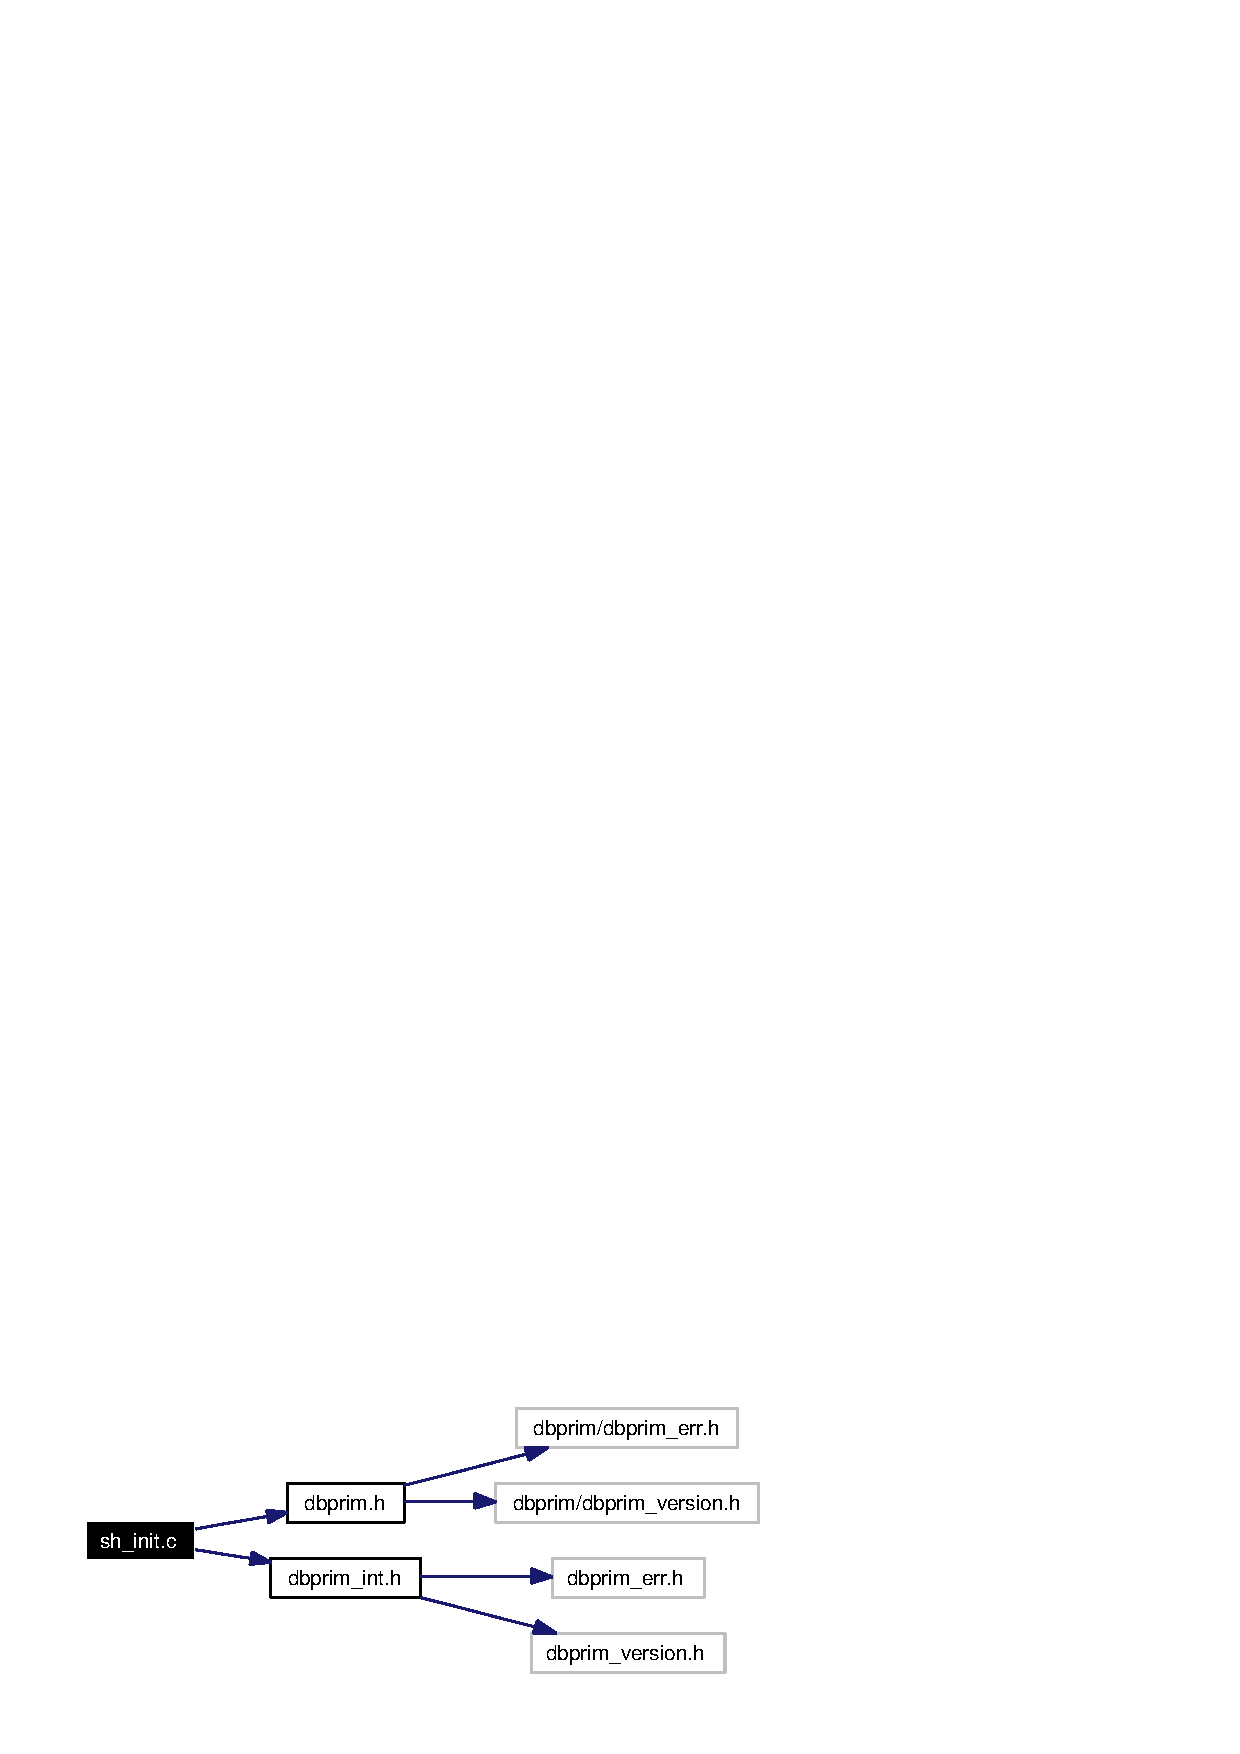
\includegraphics[width=184pt]{sh__init_8c__incl}
\end{center}
\end{figure}
\subsection*{Functions}
\begin{CompactItemize}
\item 
unsigned long \hyperlink{group__dbprim__smat_ga18}{sh\_\-init} (\hyperlink{struct__smat__head__s}{smat\_\-head\_\-t} $\ast$head, \hyperlink{group__dbprim__smat_ga6}{smat\_\-loc\_\-t} elem, void $\ast$object)
\begin{CompactList}\small\item\em Dynamically initialize a sparse matrix row or column head. \item\end{CompactList}\end{CompactItemize}
